%% Das Layout des Dokumentes wird festgelegt. Hier A4 mit einer 10er Schrift. Typ: Report 
\documentclass[a4paper,10pt,oneside]{article}

\usepackage[ngerman]{babel}
\usepackage[utf8]{inputenc}
\usepackage[T1]{fontenc}
\usepackage{amsmath}
\usepackage{graphicx} 
\usepackage{a4wide}

%%Wenn ein Absatz nicht eingerückt werden soll
\setlength{\parindent}{0cm}
 
%%Abstand zwischen Absätzen
\setlength{\parskip}{2.0ex plus 1.0ex minus 0.5ex}
 
%% das war der Vorspann, in dem die Formatierungsregeln festgelegt werden
 
%%Nun kommt das Dokument:
 
%%Anfang
\begin{document}

\tableofcontents
 
\section{Einleitung}
\subsection{Biosignale}
\begin{itemize}
	\item Chemische und elektrische Biosignale
	\item Zuständig für Steuerung, Regelung, Informationsübertragung
\end{itemize}
\subsection{Definitionen}
\begin{itemize}
	\item Biosignale: Nachrichten, die von physikalischen (oder chemischen) Aktionen des menschlichen Körpers ausgehen
	\item Biosignale: autonome, energetisch-stofflich messbare physikalische Größen
	\item Kommunikation:  Übertragung/Austausch von Informationen
	\item Interaktion: Wechselseitiges Einwirken
	\item Kooperation: Zusammenarbeit (zum gegenseitigen Nutzen)
	\item Mensch-Maschine Interaktion = M-M Kommunikation
\end{itemize}

\subsection{Arten}
\begin{itemize}
	\item Kinetische Biosignale
	\item Optische Biosignale
	\item chemische Biosignale
	\item Elektrische Biosignale
	\item Akustische Biosignale
	\item Thermische Biosignale
\end{itemize}

\subsection{Bewusste vs Unbewusste Benutzerschnittstellen}
Wichtig ist nur, dass das Biosignal reproduzierbar ist \\
Passive Schnittstelle beobachtet Benutzer und interpretiert \\
Aktive Schnittstelle = Steuerung der Maschine

\subsection{Bewertungskriterien Benutzerschnittstellen}
\begin{itemize}
	\item Effektivität (Wirksamkeit, Verlässlichkeit, Erhaltbarkeit)
	\item Effizienz (Anstrengung des Nutzers vs. benötigte Arbeitsschritte)
	\item Zufriedenheit (Bewertung durch Nutzer, kein technisches Attribut)
	\item Privatsphäre
	\item Sicherheit
	\item Flexibilität
	\item Natürlichkeit
	\item User Experience
	\item Preis
\end{itemize}

Verschiedene Sensoren zur Erfassung von Biosignalen des lebenden Organismus. \\
Ein Sensor kann mehrere Funktionen erfassen (Elektrode: EEG, EKG, EMG, EOG).

\subsection{Vor/Nachteile Biosignal basierter Benutzerschnittstellen}
Effektivität:
\begin{itemize}
	\item Robustheit (Umwelteinflüsse, Temperatur, Feuchtigkeit, Wasser, Dunkelheit etc.)
	\item Bandbreite (Nutzen unbewusster Signale vergrößert Bandbreite)
	\item Signale mit geringen Bandbreiten (EMG besser als Sprache)
	\item Throughput (Handschrift, Tippen, Sprache, Bewegung, Gestik, Mimik)
\end{itemize}
Andere Kriterien
\begin{itemize}
 \item Zufriedenheit (Tragekomfort, Bequemlichkeit)
 \item Flexibilität - Mobilität
 \item Privatsphäre (anderer und von sich selbst)
\end{itemize}

\subsection{Systemarchitektur}
\begin{itemize}
	\item Benötigt Information über Signal, Signalerfassung, Vorverarbeitung und Mustererkennung
	\item Typischer Aufbau Biosignal->Signalverarbeitung->Decoder->Adaption, wobei Applikationen, Modelle und Wissen nur auf Decoder und Adaption Einfluss nehmen
\end{itemize}

\subsection{Sprache}
\begin{itemize}
	\item Spracherkennung, Synthese, Übersetzung, Verstehen/Zusammenfassung, Sprechererkennung
	\item Z.T. Körpervibration als Biosignal verwendet für Spracherkennung, Vorteil unabhängig von Hintergrundgeräuschen
	\item Z.T. Spracherkennung über Kontraktion der Artikulationsmuskeln (lautloses Sprechen, Robust ggnüber Hintergrundgeräuschen, aber Elektroden im Gesicht)
\end{itemize}

\subsection{EEG}
\begin{itemize}
	\item Erfasst Gehirnströme
	\item Erkennt Emotionen, Mentale Auslastung, momentane Beschäftigung
\end{itemize}

\subsection{Bewegung}
\begin{itemize}
	\item Aufwändige Analyse
	\item Airwriting mithilfte von Inertialsensoren
\end{itemize}

\section{Messen von Biosignalen}

\section{11 - HMM (Hidden Markov Models)}
	\begin{itemize}
		\item Modellieren Sequenz von Datenpunkten
		\item benötigen zugrundeliegendes state modeling
		\item oft zusammen mit GMMs verwendet
	\end{itemize}
	
\subsection{Sequenzmodellierung und State-Modelierung}
	\begin{itemize}
		\item Sequenzmodellierung ist in typischer Signalverarbeitungskette letzte Schritt nach Datenverarbeitung und State Modeling 
		\item Klassifikation und Sequenzmodellierung eng miteinander verbunden
	\end{itemize}

\subsection{Dynamic Time Warping}
	\begin{itemize}
		\item einfaches Verfahren zum Vergleich von Sequenzen
		\item Algorithmen in der HMM-Modellierung sehr ähnlich zu DTW
		\item Wir haben: Aufnahmen von Sprachsignalen - Trainingsdaten (Beispielaufnahmen mit bekanntem Inhalt) + Testdaten (Aufnahmen mit unbekanntem Inhalt)
		\item Ziel: Wir wollen die Distanz einer unbekannten Sequenz und einer Beispielsequenz berechnen
		\item Frame für Frame-Vergleich Probleme: Signale sind unterschiedlich lang + Anfang und Ende der Äußerung nicht bekannt
		\item Faggot-Lösung: Lineares Alignment - für fast alle Zwecke aber viel zu unflexibel
		\item Killer-Lösung: DTW
				\begin{itemize}	
					\item basiert auf Prinzip des dynamischen Programmierens (DP) bzw. der minimalen Editierdistanz
					\item Pfade durch eine Matrix von möglichen Zuordnungen berechnet
					\item Ergebnis: Distanzmaß zwischen den beiden Äußerungen
				\end{itemize}
	
		\item Ziel: Finde Distanz zwischen den beiden Äußerungen (je niedriger desto besser)
		\item Problem: Alle Pfade müssen betrachtet werden um den Besten zu finden
		\item Lösung:
				\begin{itemize}
					\item Berechne für jede Zeit $t$ die kumulativen Distanzen $\alpha(s,t)$, die die Distanz der Teiläußerungen bis zu den Zuständen q(s,t) (s=,1,..,S)  beschreiben
					\item Die Distanzen für Zeitpunkt t+1 berechnen sich iterativ aus denen für Zeitpunkt t und hier wird Minimierung der Distanz durchgeführt
				\end{itemize}
					\item Benötige Distanzmaß $d(s,t)$ für den beobachteten Frame t und den Referenzframe s (z.B. euklidische Distanz)
 		\end{itemize}
 		\centering
 		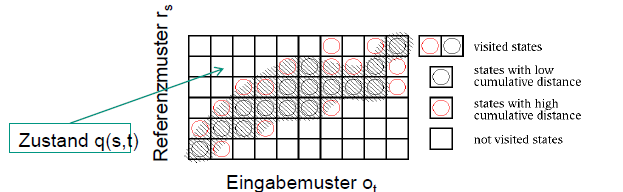
\includegraphics[scale=0.65]{Grafiken/DTW_Beispiel.png}
 		
 		\begin{itemize}
 			\item Welche Übergänge zwischen Frames sind möglich? Was haben sie für Distanz-Kosten?
 			\item Erlaubt sind überlicherweise:
 				\begin{itemize}
 					\item Ersetzung: Kosten = d(.,.) (praktisch immer > 0)
 					\item Einfügung/Auslassung eines Frames: Kosten können in der Praxis ignoriert werden
 					\item Einfügung/Auslassung mehrerer Frames: evtl. Extra-penalty, max. Zahl von Frames, die ausgelassen werden dürfen
 				\end{itemize}
 		\end{itemize}
\vspace{5px}
\flushleft Ablauf des Algorithmus:
 			\begin{itemize}
 				\item Initialisierung: Beginne bei Startzustand $q(0,0)$, $t:=0$, $\alpha(0,0):=d(0,0), \alpha(x,0)=\infty$
 				\item Für jeden Zustand $q(s,t)$:
 					\begin{itemize}
 						\item Betrachte jeden erlaubten Zustandsübergang $q(s',t-1) -> q(s,t)$
 						\item Finde min. Distanz zu $q(s,t)$
 						\item Bis Teildistanz $\alpha(s,t)$ einen gewissen Grenzwert überschreitet
 					\end{itemize}
 				\item weitere Einschränkungen des Suchraums denkbar
 				\item Komponenten der Zustandsmatrix Schritt für Schritt berechenbar (zeiteffizient + speichereffizient)
 			\end{itemize}
 		\begin{itemize}
 			\item Anwendung in der Spracherkennung
 			\item z.B. heute noch praktisch bei der Erkennung von sehr kleinen Vokabularen
		\end{itemize} 	
		
\vspace{5px}
\flushleft Probleme bei Unterscheidung einer kleinen Menge von Wörtern:
		\begin{itemize}
			\item benötigt eine Endpunktdetektion
			\item wird sehr ineffizient wenn viele Trainingsbeispiele vorhanden sind - großes Vok. braucht extrem viele Trainingsbeispiele
			\item Trainingsdaten können nicht zwischen verschiedenen Referenzen geteilt werden
			\item Erkennung unbekannter Wörter ist nicht möglich
			\item ungeeignet für kontinuierliche Sprache
			\item sehr kurze Wörter sind schwer zu trainieren
		\end{itemize}
	$\Rightarrow$ Andere Methode wird benötigt die es ermöglicht, kleinere Einheiten (Silben, Phoneme) zu trainieren und zu erkennen 		

\subsection{Markov-Modelle}
Sprachproduktion als stochastischer Prozess
	\begin{itemize}
		\item Beobachtungen zur Sprachproduktion:
		\begin{itemize}
			\item das gleiche Wort/Phonem hört sich jedesmal anders an
			\item in einem gegebenen Zustand können verschiedene Laute mit 		unterschiedlicher Wahrscheinlichkeit beobachtet werden
			\item der Produktionsprozess kann Übergänge aus einem Zustand in einen anderen machen, aber nicht alle denkbaren Übergänge sind möglich, zumindest nicht gleich wahrscheinlich
		\end{itemize}
		\item Sprachprozess befindet sich zu jedem Zeitpunkt in einem Zustand
		\item In jedem Zustand werden Laute ausgegeben entsprechend einer gewissen Wahrscheinlichkeit: Emissionswahrscheinlichkeit
		\item Die Übergänge zwischen Zuständen erfolgen auch entsprechend einer gewissen Wahrscheinlichkeitsverteilung: Übergangs- oder Transitionswahrscheinlichkeiten
		\item Markov-Modelle:
			\begin{itemize}
				\item Es gibt eine diskrete Zustandsmenge ${s_1, ... ,s_N}$
				\item Wir beobachten eine probabilistische Zustandssequenz $O = (o_1,...,o_T), o_i \in  {1,...,N}$
				\item Markov-Annahme: Wahrscheinlich, dass wir zum Zeitpunkt t in einem gewissen Zustand sind, hängt nur von vorhergehendem Zustand ab
				\item Verteilung soll stationär (zeitunabhängig) sein
			\end{itemize}
	\end{itemize}
	
\subsection{Hidden-Markov-Modelle}
Markov-Modelle und Spracherkennung
	\begin{itemize}
		\item Zustand $<=>$ Beobachtung
		\item In der Sprache haben wir aber ein Kontinuum an möglichen Tokens (typischerweise Sprachsignalframes), die endlich vielen Zuständen (Phonemen) zugeordnet werden sollen
		\item In der Sprache sind die Zustände versteckt (hidden)
	\end{itemize}
	
Hidden-Markov-Modelle (HMM) 
	\begin{itemize}
		\item sind ein doppelter stochastischer Prozess
			\begin{itemize}
				\item Zustandsabfolge probabilistisch
				\item Jeder Zustand emittiert seine Beobachtung: Diese Emission ist ebenfalls probabilistisch
				\item Zustandsfolge ist versteck (hidden)
			\end{itemize}
		\item Sind Markov-Modelle (1. Ordnung)
			\begin{itemize}
				\item Wahrscheinlichkeiten für den Eintritt in den nächsten Zustand hängen nur vom aktuellen Zustand ab
			\end{itemize}
		\item Nichtbeobachtbarkeit der Zustandsfolge hat eine Reihe von Konsequenzen		
			\begin{itemize}
				\item Sprachdekodierung mit HMMs: Anhand der Beobachtungen auf eine mögliche Zustandssequenz rückschließen (dabei wird man nie die exakte Lösung erhalten, sondern nur eine mit höchster Wahrscheinlichkeit)
				\item Training von HMMs: Kennen zwar die durchlaufene Zustandsfolge, aber nicht die Zeitpunkte der Zustandsübergänge
			\end{itemize}
			\centering 
			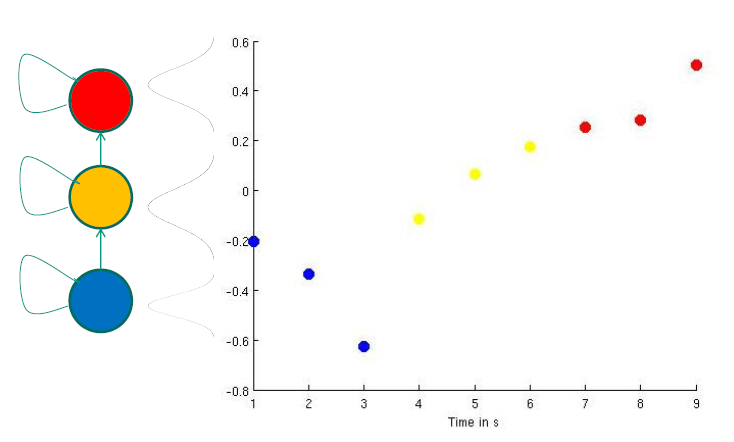
\includegraphics[scale=0.5]{Grafiken/hmm-darstellung.png}
	\end{itemize}

Formale Definition:
	\begin{itemize}
		\item HMM $\lambda = (S,\pi, A,B,V)$
		\item $S={s_1,...,s_N}$ - Menge aller möglichen Zustände
		\item $\pi$: $\pi(s_i) = P(q_1 = s_i)$ - Anfangsverteilung bei t=1
		\item $A=((a_{ij})), 1 \leq i, j \leq n$ - Matrix von Übergangswahrscheinlichkeiten
		\item $B=(b_i)$ - Vektor von Ausgabewahrscheinlichkeiten, d.h. $b_i(v)=P(o_t = v | q_t = s_i)$. Dabei ist $v \in V$
		\item V - Vokabular, Menge der Ausgabesymbole (diskret oder kontinuierlich)
	\end{itemize}

Diskrete HMMs:$V = {x_1,x_2, ...,x_v}$, dann sind die $b_i$ diskrete Wahrscheinlichkeiten


Kontinuierliche HMMs: $V=R^d$, dann sind die $b_i$ stetige Wahrscheinlichkeitsdichten

\begin{itemize}
	\item Für die Anfangswahrscheinlichkeiten gilt $\sum_i \pi(s_i) = 1$. Vereinfachend nimmt man oft einfach: $\pi(s_1) = 1 \enspace , \enspace \pi(s_j) = 0 \enspace , \enspace j \neq 0$, d.h. es gibt einen ausgezeichneten Startzustand)
	\item Es gilt $\sum_j a_{ij} = 1$ für alle i und meistens ist $a_{ij} = 0$ für die meisten Folgezustände j
\end{itemize}
Die Struktur eines HMMs nennt man Topologie:
	\begin{itemize}
		\item Lineares Modell:  \\ 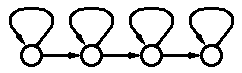
\includegraphics[scale=0.3]{Grafiken/hmm-struktur.png} 
		\item Links-nach-Rechts-Modell: \\ 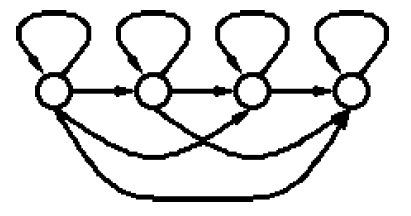
\includegraphics[scale=0.2]{Grafiken/hmm-lnr.png} 
		\item Alternative Pfade: \\ 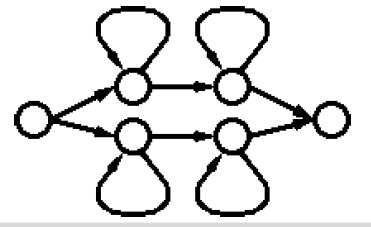
\includegraphics[scale=0.2]{Grafiken/hmm-ap.png}
		\item Bakis model (lin. Modell + kann je 1 Zustand übersprungen werden): \\ 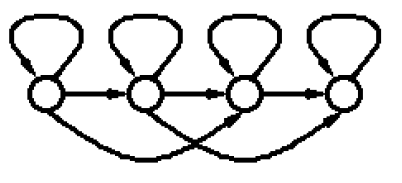
\includegraphics[scale=0.2]{Grafiken/hmm-bakis.png}   
		\item Ergodisches Modell (Jeder Zustand ist von jedem anderen Zustand erreichbar): \\
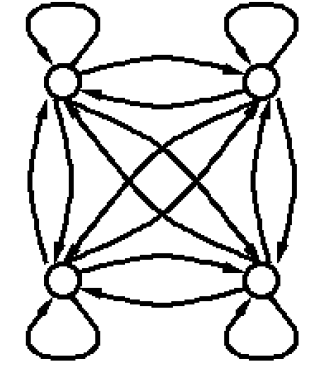
\includegraphics[scale=0.2]{Grafiken/hmm-em.png} 
	\end{itemize}

HMM-Theorie kennt drei Hauptaufgaben: Evaluationsproblem, Dekodierungsproblem, Optimierungsproblem

Evalutationsproblem: Berechne die Wahrscheinlichkeit der Beobachtung $P(O|\lambda)$
	\begin{itemize}
		\item Entspricht der Durchführung des DTW-Algorithmus
		\item Forward-Algorithmus löst dieses Problem
		\item Herausforderung: Wir müssen die Wahrscheinlichkeit der Beobachtung entlang aller möglichen Pfade berechnen
		\item Sehr aufwendig - Finden effizienter Algorithmen
		\item Frage: Wie summieren wir die Wahrscheinlichkeiten entlang aller möglichen Pfade effizient auf?
		\item Lösung: Ansatz ist wie beim dyn. Programmieren:
			\begin{itemize}
				\item Berechne iterativ für jeden Frame und jeden Zustand die Vorwärts-Teilwahrscheinlichkeiten (forward probabilities) $\alpha$
				\item Dann ergibt sich eine Matrix A der Vorwärtswahrscheinlichkeiten \\ 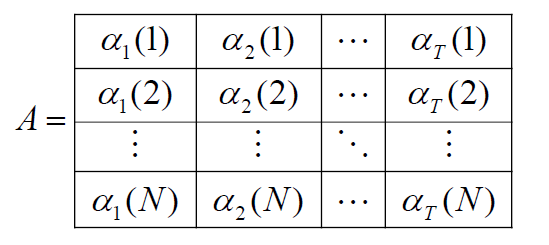
\includegraphics[scale=0.2]{Grafiken/hmm-fa-A.png}
				\item $\alpha_t(j)$ bezeichnet die Wahrscheinlichkeit, bei gegebener Teilbeobachtung zum Zeitpunkt t im Zustand j zu sein. Zur Berechnung iteriert man über die Zeit:
				\item Init: $\alpha_1(j) = b_j(o_1) \pi(s_j)$
				\item Induktion: $\alpha_t(j) = b_j(o_t) \cdot \sum_{i=1..n} a_{ij} \alpha_{t-1}(i)$ 
				\item Ergebnis: $p(o_1,o_2,...,o_T|\lambda) = \sum_{j=1..n} \alpha_T(j)$
				\item Komplexität: $O(N^2T)$
			\end{itemize}
	\end{itemize}

Dekodierungsproblem: Berechne die wahrscheinlichste Zustandsfolge bei der gegebenen Beobachtung $(q_1^*,...,q_{t-1}^*,q_t^*) = arg \max_{q_1,...,q_t} P(q_1,...,q_t|O,\lambda)$. Viterbi-Algorithmus:
	\begin{itemize}
		\item Definiere: $z_t(j) := \max_{q_1,...,q_{t-1}} P(q_1,...,q_{t-1}, q_t = j, o_1,...,o_t)$
		\item $z_t$ ist die maximale Wahrscheinlichkeit (maximiert über alle Zustandsfolgen bis Zeitpunkt t), mit der bei der gegebenen Teilbeobachtung zum Zeitpunkt t der Zustand j erreicht wird
		\item Man kann $z_t(j)$ iterativ berechnen, indem man alle möglichen Vorgängerzustände betrachtet und maximiert: \\
			$z_t(j) = \max_i z_{t-1}(i) \cdot a_{ij} \cdot b_j(o_t)$\\
			$z_1(j) = \pi(s_j) \cdot b_j(o_1)$
		\item Ergibt sich eine Matrix Z, ähnlich wie beim Forward-Algorithmus \\
		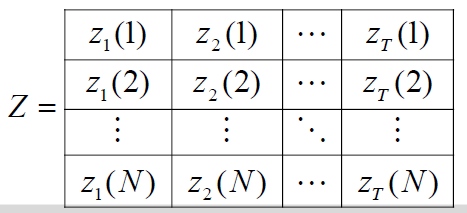
\includegraphics[scale=0.2]{Grafiken/viterbi-algo.png}
		\item Rechenaufwand: $O(N^2T)$
		\item Außerdem speichern wir für jeden Zustand den optimalen Vorgängerzustand: $r_t(j) = argmax_t (z_{t-1}(i) a_{ij})$
		\item Wenn alle $z_t$ und $r_t$ berechnet sind, kann Rückwärtszeiger $r_t$ benutzt werden, um die gesuchte optimale Zustandsfolge zu berechnen
		\item Beginne beim letzten Zeitpunkt T und suche den wahrscheinlichsten Zustand. Dann gehe entlang der Rückwärtszeiger schrittweise zurück: \\
		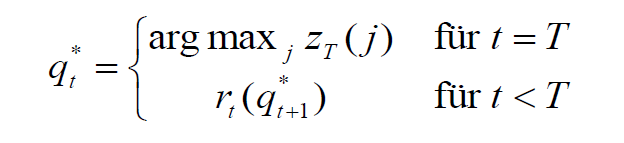
\includegraphics[scale=0.2]{Grafiken/viterbi-algo-qt.png}
	\end{itemize}

Optimierungsproblem: Finde ein HMM $\lambda^{'}$, so dass $P(O|\lambda^{'})> P(O|\lambda)$ (Ein gegebenens HMM $\lambda$ soll verbessert werden)
	\begin{itemize}
		\item Welche Parameter können trainiert werden: Übergangswahr., Emissionswahr., Anfangswahr.
		\item Probleme bei der Optimierung: unbekannt zu welchem Zeitpunkt wir in welchem Zustand sind, Wahrscheinlichkeit berechenbar dass zu Zeitpunkt t im Zustand $s_j$ (diese Information können wir zur Gewichtung nutzen)
		\item Lösung des Optimierungsproblem besteht aus 2 Schritten:
		\item Estimation Step: Berechne die Zuordnungswahrscheinlichkeit von Trainingsdaten zu HMM-Zuständen
			\begin{itemize}
				\item Trainingsbeobachtung $O=(o_1,...,o_T)$
				\item für jedes Sample die Wahrscheinlichkeit berechnen, dass es einem gewissen HMM-Zustand zuzuordnen ist
				\item für jede Kombination von aufeinanderfolgenden Samples die Wahrscheinlichkeit berechnen, dass sie einem gewissen Zustandsübergang zuzuordnen sind
			\end{itemize}
		\item Maximization Step: Optimiere die Parameter von Emissionswahrscheinlichkeiten, (Übergangswahrscheinlichkeiten und Anfangswahrscheinlichkeiten)
	\end{itemize}
 
Forward-Backward-Algorithmus:
	\begin{itemize}
		\item Berechnet die Zuordnungswahrscheinlichkeiten von Trainingsdaten zu HMM-Zuständen, löst also den Expectiation Step
		\item Betrachten wir eine Beobachtung $o=(o_1,...,o_T)$
		\item Gesucht sind 2 Parameter:
			\begin{itemize}
				\item $Y_t(j) = P (q_t=j|o_1,...,o_T,\lambda)$ ist die Wahrscheinlichkeit, dass der Beobachtungsvektor $o_t$ zum Zustand j gehört
				\item $\xi_t(i,j) = P (q_t=i,q_{t+1}=j | o_1,...,o_T,\lambda)$ ist die Wahrscheinlichkeit, dass zum Zeitpunkt t im Zustand i befinden und dann in den Zustand j übergehen
			\end{itemize}
		\item Beide Wahrscheinlichkeiten hängen von der gesamten Beobachtung o ab
		\item Berechnung von $y$ und $\xi$
			\begin{itemize}
				\item Forward-Algorithmus berechnet die Wahrscheinlichkeit, nach der Teilbeobachtung $(o_1,...,o_t)$ also zum Zeitpunkt t im Zustand j zu sein
				\item Backward-Algorithmus berechnet die Wahrscheinlichkeiten im Zustand j zu sein und dann die Teilbeobachtung $(o_{t+1},...,o_T)$ zu machen
				\item Kombination der beiden ergibt Forward-Backward-Algorithmus, der $Y_t(j)$ berechnet
				\item Berechne $P(q_t=j|o_1,...,o_T,\lambda)$ druch Aufspaltung in Forward-Teil (bis Zeit t) und Backward-Teil (nach Zeit t).
				\item $\alpha_t(j) := P(q_t=j,o_1,...,o_t|\lambda)$ \\
					  $\beta_t(j) := P(q_{t+1}=j,o_1,...,o_T|\lambda)$ \\
					  $\Rightarrow P(q_t=j|o_1,...,o_T,\lambda) = \alpha_t(j) \cdot  \beta_t(j)$. Anwendung der Bayes-Regel ergibt: \\ \vspace{3px}
				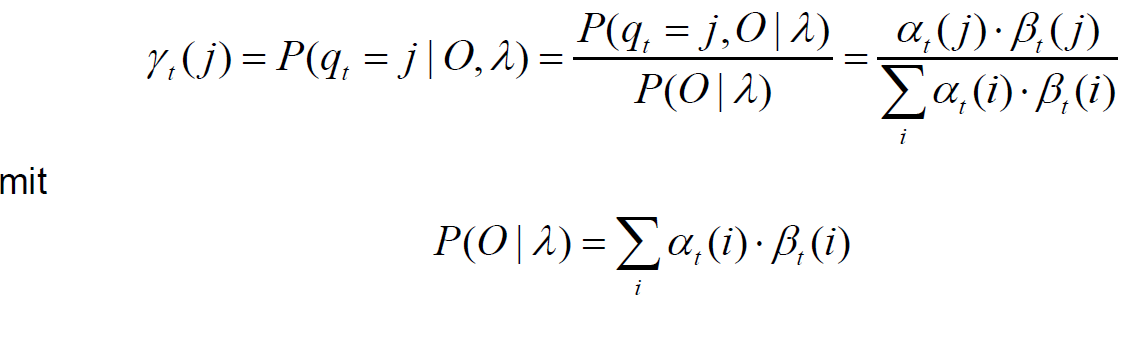
\includegraphics[scale=0.2]{Grafiken/forward-backward-algo.png}	  	
				\item $\beta_t$ können ähnlich wie die $\alpha_t$ rekursiv berechnet werden, aber rückwärts:
					\begin{itemize}
						\item Init: $\beta_T(i) = 1$ für alle Zustände i
						\item Induktion: $\beta_t(t) = \sum_{j=1..n} a_{ij} b_j (o_{t+1})\beta_{t+1}(j), \enspace t=T-1,..., 1$
						\item Durch Aufsummieren: $\Rightarrow p(o_{t+1},o_{t+2},...,o_T|\lambda) = \sum_{j=1..n} \beta_T(j)$
					\end{itemize}			
				\item[] 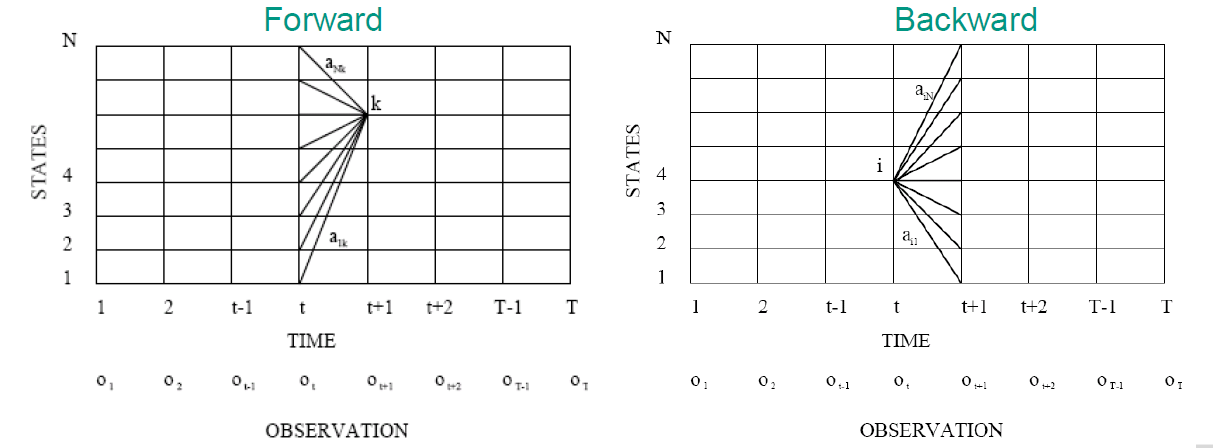
\includegraphics[scale=0.25]{Grafiken/forward-backward-beta.png}	  		 		\item $\xi_t(i,j)$: auch mit Forward-Backward-Algorithmus $\xi_t(i,j) = P(q_t = i,q_{t+1} = j|O,\lambda)$
				\item[] 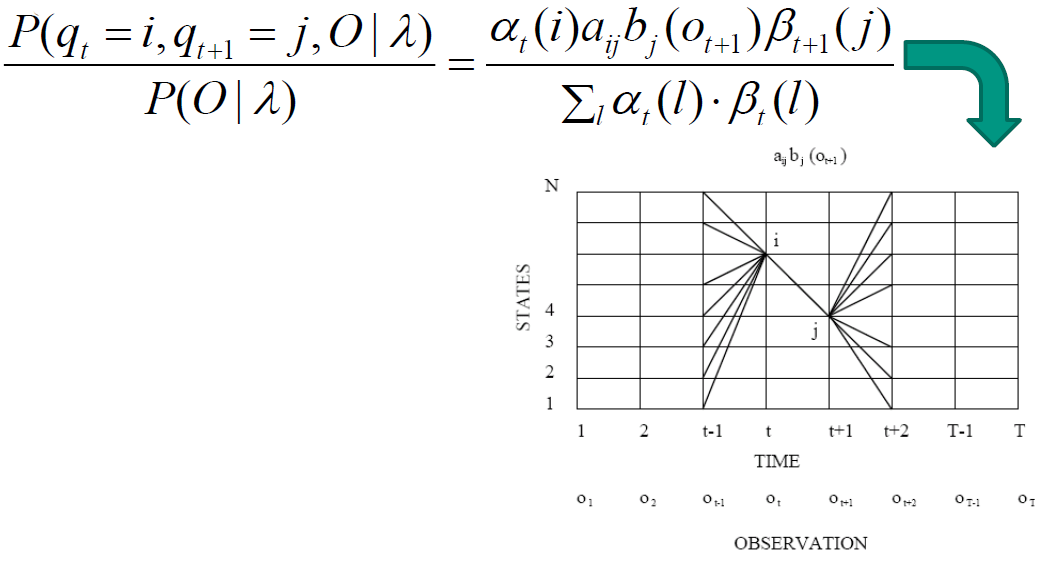
\includegraphics[scale=0.2]{Grafiken/xis.png}
			\end{itemize}
	\end{itemize}

\underline{Optimierung des HMMs:}
	\begin{itemize}
		\item Trainingsdaten den HMM-Zuständen und Zustandsübergängen zugeordnet
		\item Das war der Expectation Step des Algorithmus
		\item Führe nun Maximierung der HMM-Ausgabewahrscheinlichkeit durch (Maximization Step)
		\item Zuordnung der Samples zu HMM-Zuständen, gegeben durch $\alpha_t(j),\beta_t(j),Y_(j)$
		\item Falls Emissionswahrscheinlichkeiten durch Gauss-Mischverteilungen modellieren, dann verwende EM-Algorithmus zum Training
	\end{itemize}
	
\underline{Optimierung der Emissionswahrscheinlichkeiten:} \\
Betrachten Emissionswahrscheinlichkeiten $B^{'}=(b_1^{'},...,b_N^{'})$ bei diskretem Ausgabealphabet V. Zu jedem Zustand i = 1,...,N gehört eine Verteilung $b_i$, so dass $b_i(v_k) \in  [0,1]$ die Wahrscheinlichkeit angibt im Zustand i die Beobachtung $v_k$ zu machen. \\
Danach werden die $b_i^{'}$ bestimmt: 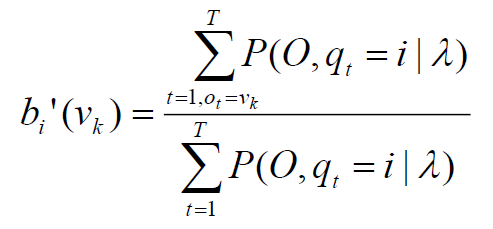
\includegraphics[scale=0.2]{Grafiken/bis.png}\\
Das heißt, $b_i^{'}(v_k)$ entspricht dem Anteil der Emissionen von $v_k$ an der Gesamtzahl der "Besuche" von Zustand i.
	
	
\underline{Optimierung der Übergangswahrscheinlichkeiten:} 	
	\begin{itemize}
		\item $sum_{t=1..T-1} \xi_t(i,j)$ ist der Erwartungswert der Anzahl der Transitionen von i nach j
		\item Der neue Wert $a_{ij}^{'}$ ist der Anteil der Transitionen von i nach j, normalisiert durch die Gesamtzahl der Transitionen (=Besuche) von i 
		\item Summiere über alle Zeitpunkte t=1,...,T: $a_{ij}^{'} = \frac{\sum_t \xi_t(i,j)}{\sum_t \gamma_t(i)}$
		\item Der neue Wert $\pi^{'}(i)$ ist dementsprechend die Anzahl der Besuche von i zur Zeit t = 1, also $\pi_t^{'} = \gamma_1(i) = \frac{\alpha_1(i)\beta_1(i)}{\sum_l \alpha_1(l)\beta_1(l)}$
	\end{itemize}
 		
\underline{Baum-Welch-Regeln:} \\ 	
	\begin{itemize}
		\item Alle Parameter des HMMs an die aktuelle probabilistische Zuordnung der Samples, gegeben durch $\gamma_t(i)$, angepasst. Es ergibt sich also ein neues HMM: $\lambda^{'} = (S,\pi^{'},A^{'},B^{'},V)$
		\item Dieser Algorithmus wird, wie es für EM-Algorithmen typisch ist, so lange iterativ wiederholt, bis ein Abbruchkriterium erfüllt ist
		\item Die Regeln der letzten "Folien" sind die Baum-Welch-Regeln
	\end{itemize}
	
\underline{Training von HMMs mit Viterbi:} \\ 
	\begin{itemize}
		\item Viterbi, der immer nur maximale Wahrscheinlichkeiten betrachtet, geht viel schneller als Forward-Backward-Algorithmus
		\item In der Spracherkennung ist Viterbi-Training Standard
	\end{itemize}
	
\section{12 - Spracherkennung}
\subsection{Schall als Luftdruckwelle} 

\underline{Was ist Schall?} \\ 
	\begin{itemize}
		\item Druckwelle, die von einem vibrierenden Objekt erzeugt wird
		\item Vibration überträgt sich auf Partikel des umgebenden Trägermediums (z.B. Luft) - Energietransport über Medium findet statt
		\item Partikel parallel zur Ausbreitungsrichtung der Welle - spricht man von Longitudinalwelle
		\item Longitudinalwelle besteht aus Kompressionen (Verdichtungen) + Rarefaktionen (Verdünnungen) der Luft
		\item Lässt sich durch Sinusfkt. beschreiben
		\item Amplitude entspricht der Dichte der Luft an der betreffenden Stelle
		\item Ausbreitungsgeschwindigkeit in der Luft: 331,5 + 0,6 T m/s, T = Temperatur in C
	\end{itemize}

\underline{Messung der Schallintensität} \\  
 	\begin{itemize}
 		\item leseste hörbare Ton moduliert den Luftdruck um etwa $10^{-5} Pa$, Schmerzgrenze: $100 = 10^2 Pa$
 		\item Wird in Dezibel [dB] gemessen (dB ist Verhältnis von zwei Schallintensitäten)
 		\item Schalldruckpegel (sound pressure level, SPL) misst den absoluten Schalldruck in dB
 		\item Referenzgröße $P_0$ ist die Hörschwelle von $2 \cdot 10^{-5} Pa$ $SPL = 20 \cdot log_{10} (P / P_0)$
 	\end{itemize}
 
\subsection{Der menschliche Sprachproduktionsapparat} 
\underline{Sprachproduktionsapparat} \\ 		
 	\begin{itemize}
 		\item Sprache besteht aus Luftdruckwellen - diese werden von Mund und Nase ausgestoßen
 		\item Erzeugung dieser Wellenform besteht aus 2 Schritten
 			\begin{itemize}
 				\item Stimmbänder und Kehlkopf erzeugen eine Grunderregung
 				\item Der Dokaltrakt (Mundhöhle, Nasaltrakt) wirkt als ein Filter auf diese Grunderregung und moduliert sie
 			\end{itemize}
 		\item Grunderregung kann eine periodische Schwingung oder aperiodisches Rauschen sein
 		\item Häufige Annahme: Erregung und Filter sind unabhängig
 	\end{itemize}
 
\underline{Grundfrequenz} \\
Betrachten wir zuerst den Fall, dass die Stimmbänder sich öffnen und schließen und so die Grunderregung erzeugen
	\begin{itemize}	
		\item Periodisches öffnen und schließen der Stimmbänder erzeugt periodische Schwingung (Grunderregung)
		\item Dauer eine Periode hängt von Länge und Anspannung der Stimmbänder und dem von der Lunge erzeugten Luftdruck ab
		\item Die Periode kann vom Sprecher in gewissen Grenzen moduliert werden, um die Tonhöhe (pitch) zu modulieren
		\item Öffnungszyklus der Stimmbänder:
			\begin{itemize}
				\item Stimmbänder widerstehen dem Lungenluftdruck
				\item Unter immer stärkerem Druck öffnen sich die Stimmbänder
				\item Wenn der Druck wieder gering ist fallen die elastischen Stimmbänder wieder in die Ausgangsposition
			\end{itemize}
		\item Anzahl dieser Öffnungsvorgänge pro Sekunde als Grundfrequenz der Sprache $f_0$
		\item Variiert von 60 Hz (große Männer) bis 300 Hz (Kinder)
		\item Grundfrequenz bestimmt die Periode für die höherfrequenten harmonischen Schwingungen des Vokaltrakts
	\end{itemize}
	
\underline{Stimmhafte vs. stimmlose Phoneme} \\
	\begin{itemize}
 		\item Laute sind stimmhaft, wenn während der Artikulation eine Vibration der Stimmbänder vorliegt
 		\item Andernfalls sind die Stimmbänder geöffnet, und die Grundanregung des Lautes ist ein Rauschen mit gewissen chaotischen Eigenschaften
 		\item Beispiel für beide Lautarten: Wellenform des engl. Wortes sees \\
 		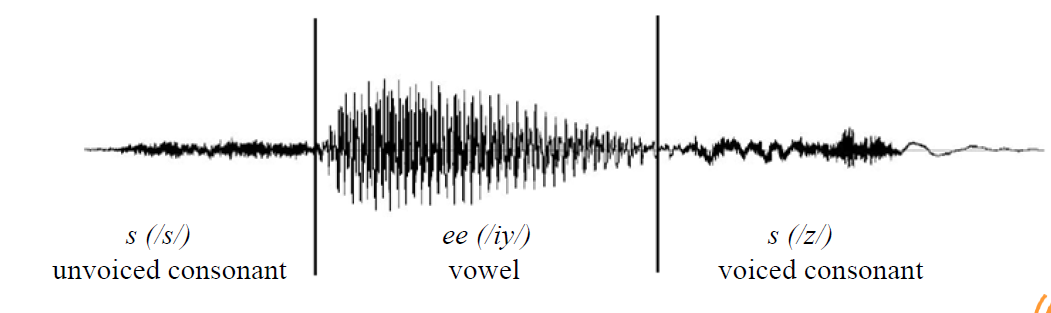
\includegraphics[scale=0.2]{Grafiken/bsp-sees.png}
	\end{itemize}
 		
\underline{Das Quelle-Filter-Modell} \\
	\begin{itemize}
		\item Wellengenerator: Periodische Schwingung der Stimmbänder
		\item Rauschgenerator: Luftstrom bei stimmlosen Phonen
		\item Systemmodell: Filtereigenschaft des Vokaltraktes (Mundraums)
		\item[] 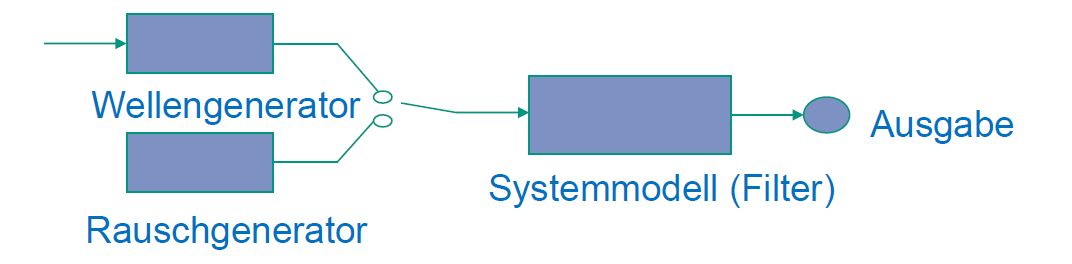
\includegraphics[scale=0.2]{Grafiken/quelle-filter-modell.png}
	\end{itemize}

\subsection{Akustische Phonetik und Phonologie}
\underline{Phonetik und Phonologie} \\
	\begin{itemize}
		\item Phonetik: Studium der Produktion, Klassifikation und Transkriptiopn von Sprachlauten -> Fokus liegt auf der akustischen Realisierung der Sprachlaute
		\item Phonologie: Studium der Verteilung und Struktur von Lauten in einer Sprache -> Hauptziel ist es, übergreifende Charakteristiken von Sprachlauten zu finden
	\end{itemize}

\underline{Phonetik} \\
	\begin{itemize}
		\item Artikulatorische Eigenschafen
			\begin{itemize}
				\item Laute können neben stimmhaft/stimmlos nach artikulatorischen Eigenschaften unterschieden werden
				\item Unterscheidung erfolgt entsprechend der Anatomie der wichtigen Artikulatoren und ihrer Position im Vokaltrakt
				\item Hauptkomponenten des menschl. Sprachproduk.apparats: Lungen, Trachea (Luftröhre), Pharynx (Rachen), Nasenhöhle und Mundhöhle. (Rachen + Mundhöhle = Vokaltrakt, Nasenhöhle = Nasaltrakt)
				\item Innerhalb des Vokaltrakts sind Stimmbänder, weicher Gaumen (Velum), harter Gaumen (Palatum), Zunge, Zähne und Lippen
			\end{itemize}
		\item Benennung von Sprachlauten
			\begin{itemize}
				\item Nasallaute:Luftstrom hauptsächlich durch Nase, gesenktes Velum (/n/)
				\item Orallaute: Luftstrom durch Mund, Velum verschließt Nasalraum
				\item Stoplaute (Plosive):Vokaltrakt kurzzeitig vollst. verschlossen (/p/, /b/)
				\item Frikative: Vokaltrakt teilw. verschlossen, Reibung entsteht (/f/)
				\item Approximanten: Vokaltrakt verengt, keine Reibung (/j/)
				\item Labial: Artikulationsort Lippen (/b/, /w/)
				\item Dental: Artikulation Zunge an Zähnen
				\item Alveolar: Alveole (Zahndamm) aktiv
				\item Palatal: Harter (vorderer) Gaumen aktiv
				\item Velar: Weicher (hinterer) Gaumen aktiv
				\item Glottal: Glottis, Stimmbänder aktiv (z.B. Be-amte)			
			\end{itemize}
		\item Konsonanten und Vokale
			\begin{itemize}
				\item Bei der Artikulation von Konsonanten befindet sich irgendwo im Vokaltrakt ein Hindernis (Stop, Verengung) für den Luftstrom
				\item Bei Vokalen liegt kein solches Hindernis vor
				\item Wichtige Eigenschaften für die Spracherkennung wichtig:
					\begin{itemize}
						\item Durschnittliche Dauer von Vokal ist viel länger als von Konsonant
						\item Vokale tragen den Hauptteil an Energie im Signal
						\item => Vokale wichtig für Spracherkennung, Konsonanten sind schwach und können mit Stille verwechselt werden
						\item Bei (englischem/deutschem) Text ist es gerade andersherum
					\end{itemize}
			\end{itemize}
		\item Modell des menschlichen Vokaltrakts
			\begin{itemize}
				\item Menschliche Vokaltrakt kann durch eine verlustfreie Röhre mit variablem Querschnitt approximiert werden
				\item Wichtige Approximation: Verkettung von endlichen vielen Röhren mit festen Querschnitt
				\item Mit dem Modell berechnen sich die Filereigenschaften des Vokaltrakts
				\item [] %G 12 - 18
			\end{itemize}
		\item Mathematische Beschreibung
			\begin{itemize}
				\item Unter geeigneten Bedingungen erfüllen Schallenwellen im Vokaltrakt die linearen partiellen DGLs
				\item "lossless tube"-Modell mit N Röhren approx. A
				\item analytische Lösung der DGLs möglich => Approximation der Frequenzantwort des Vokaltraktes
				\item Dieser Filter hat i.a. N konjugiert-komplexe Polstellen, die N/2 Resonanzfrequenzen (Formanten) entsprechen
				\item Tonhöhe der Formanten definieren den Laut
				\item Vokaltraktfilter kann durch ein nur-Pole-Modell, das nur Resonanzfrequenzen berücksichtigt, schon gut modelliert werden
			\end{itemize}
		\item Eigenschaften des Sprachspektrum
			\begin{itemize}
				\item Im Spektrum des Sprachsignals sind die Oberfrequenzen der Anregungsschwingung, die von den Stimmbändern kommt, besonders stark vertreten, so dass das Spektrum selber annährend periodisch ist
				\item Vokaltrakt wirkt als Filter auf die Anregung
			\end{itemize}
		\item Formanten
			\begin{itemize}
				\item Formanten lassen sich aus Spektrogrammen ablesen
				\item Die ersten beiden Formanten bestimmen im wesentlichen den Klang eines Vokals
			\end{itemize}
		\item Klassifikation von Vokalen: Formanten
			\begin{itemize}
				\item Das Vokaldreieck gibt an, welche Vokale im Mittel welche Formanten haben
				\item[] %G 12 - 23 rechts
			\end{itemize}
		\item Klassifikation von Vokalen: Formanten F1 und F2
			\begin{itemize}
				\item F1 entspricht der Hauptresonanzfrequenz des Rachenraumes
				\item F2 ist die Hauptresonanzfrequenz des Mundraumes
				\item Weg von Kehlkopf bis zur Zunge ist länger als Weg von Zunge bis Lippen => F1 < F2
				\item Zungenposition und Mundraum bestimmen die Werte F1 und F2
			\end{itemize}
		\item Diphtonge - Die charakteristischen Formanten F1 und F2 heißen auch formant targets, wenn
			\begin{itemize}
				\item Vokal ein spezifisches Ziel hat - Monophthong
				\item Zwei verschiedene Ziele kombinieren - Diphtonge
				\item Gibt einen fließenden Übergang zwischen den beiden Zielen
				\item Manche Sprachen (z.B. Mandarin) haben sogar Triphthonge 
				\item Diphtong wird i.d.R. genauso lang gesprochen wie ein Monophthong
			\end{itemize}
		\item Klassifikation von Konsonanten
			\begin{itemize}
				\item Werden durch Art und Ort der Artikulation beschrieben
				\item Artikulationsart - Mechanismus mit dem die Artikulation passiert
				\item Artikulationsort - Beschreibt Ort der Hauptverengung
				\item Sonorität (Schallfülle), Stimmhaftigkeit, Aspiration, Stärke
			\end{itemize}
		\item Vokaltraktformen: Plosive (Verschlusslaute)
			\begin{itemize}
				\item[] %G 12 - 28 + Spektogramm
				\item weiteres Plosiv: Glottal stop (Glottisschlag, Glottisverschlusslaut) - Luftstrom von den Stimmbändern im Kehlkopf gestoppt 
				\item Typisch: Kurzzeitig Luftstrom völlig unterbrochen
			\end{itemize}
		\item Vokaltraktformen: Nasale
			\begin{itemize}
				\item[] %G 12 - 13 +Spektogramm
				\item Mundraum komplett abgeschlossen und Rachenraum und Nasaltrakt miteinander verbunden
				\item Markante Eigenschaft: auffälligen fehlenden Frequenzbänder (gewisse Frequenzen im Mundraum werden vollständig reflektiert und so löschen sich Wellen aus)
			\end{itemize}
		\item Vokaltraktformen: Frikative (Reibelaute)
			\begin{itemize}
				\item[] %G 12 - 32 +Spektogramm
				\item Desweiteren gibt es glottalen Frikativ /h/ (wie in Haus) 
			\end{itemize}
		\item Phone und Phoneme
			\begin{itemize}
				\item Zwischen Schreibweise eines sprachl. Lautes und seiner Aussprache gibt es (prinzipiell) keinen Zusammenhang
				\item Phonetik: Sprachlaute haben keine inhärente Bedeutung
				\item Phonem: Kleinste Spracheinheit, die ein Wortpaar unterscheidet (minimales Paar) - Bsp: /kind/ != /rind/ -> /k/ und /r/ sind Phoneme
				\item Phon: Belieber Sprachlaut, der von anderen Sprachlauten akustisch unterschieden werden kann 
				\item Mit Phonem ist ein Bedeutungsunterschied verbunden und mit Phon nur ein akustischer Unterschied
				\item Schreibkonvention: /phonem/ vs [phon]
			\end{itemize}
		\item Phonetische Alphabete
			\begin{itemize}
				\item IPA: International Phonetic Alphabet (von der International Phonetic Association entwickelt + enthält Inventar für alle Laute aller Sprachen der Welt)
				\item Worldbet: 1-1 Abbildung von IPA-Symbolen auf ASCII-7 Symbole, um IPA-Alphabet auf Computern nutzbar zu machen
				\item Klein- und Großschreibung von Buchstaben hat auch Bedeutung
				\item Sampa: Basiert auch auf ASCII-7 Symbolen, wurde aber ursprünglich nur die deutsche und dann Indoeuropäische Sprachen entwickelt + Kürzlich auch auf weitere Sprachen ausgedehnt (X-Sampa)
			\end{itemize}
		\item IPA-Schema für Konsonanten + Vokale
			\begin{itemize}
				\item[] Konsonanten: %G 12 - 38
				\item[] Vokale: %G 12 - 39
			\end{itemize}
		\item Phone und Phoneme 
			\begin{itemize}
				\item Phoneme unterscheiden sich in Aussprachen durch:
					\begin{itemize}
						\item 1. Koartikulation, Kontext
						\item 2. Koartikulation bei variabler Sprechgeschwindigkeit
					\end{itemize}
				\item Wenn es mehrere Phone gibt, die dasselbe Phonem repräsentieren - heißt dann Allophone
			\end{itemize}
		\item Koartikulation
			\begin{itemize}
				\item Phoneme werden of auf systematische Weise von ihren Nachbarphonen beeinflusst
				\item Diesen Prozess bezeichnet man als Koartikulation
				\item In kontinuierlicher Sprache (mit variabler Sprechgeschwindigkeit)
					\begin{itemize}
						\item werden formant targets macnhmal nicht vollständig erreicht
						\item Betonungsmuster können verändert sein
						\item Laute können modifiziert werden (Assimilation)
						\item Laute können ganz verschwinden (Elision)
					\end{itemize}
				\item Effizientprinzip
					\begin{itemize}
						\item Sprecher versucht, den artikulatorischen Aufwand zu minimieren, ohne das dabei Information verlorengeht 
						\item Sprecher kann je nach Situation seinen Sprechgeschwindigkeit erhöhen 
					\end{itemize}
				\item Laute innerhalb einer Silbe beeinflussen sich mehr als benachbarte Laute in verschiedenen Silben
			\end{itemize}
		\item Prosodie 
			\begin{itemize}
				\item Eine Phrase kann, von der Intonation einzelner Laute abgesehen, auch als ganzes eine Melodie haben
				\item Eine Prosodie enthält Information über: Intention der Äußerung, Relevanz, Auflösung syntaktischen oder semantischen Zweideutigkeiten, Emotionen des Sprechers
				\item Prosodische Information ist: Intonation ("Melodie" des Satzes), Pausen, Betonung, Rhythmus
			\end{itemize}
	\end{itemize}

\subsection{Sprachperzeption}
\underline{Sprachproduktion und Sprachperzeption} \\
	\begin{itemize}
		\item Akustische Sprache pflanzt sich dann als Schalldruckwelle durch die Luft fort und wird vom menschlichen Ohr oder Mikrofon aufgefangen
	\end{itemize}
	
\underline{Sprachkommunikation von Mensch zu Mensch} \\
	\begin{itemize}
		\item[] %G 12 - 46
		\item A: Neurophysiologischer Prozess im Gehirn
		\item B: elek. Prozess in den efferenten Nervenbahnen
		\item C: Bewegung des Artikulationsapparates
		\item D: Erzeugung des akustischen Sprachsignals im Vokaltrakt
		\item E: Akustische Übertragung des Sprachsignals
		\item F: mechanischer Prozess im Mittelohr, hydromechanischer Prozess im Innenohr
		\item G: elek. Signale in den afferenten Nervenbahnen
		\item H: Neurophysiologischer Prozess im Gehirn des Empfängers
		\item I: Akustisches Feedback zum Ohr des Sprechers
	\end{itemize}
	
\underline{Physiologie des Ohres} \\
	\begin{itemize}
		\item Ohr empfängt die Schalldruckwellen aus der Luft
		\item Drucksignal wird in elek. Signal umgewandelt
		\item elek. Signal wird zum Gehirn weitergeleitet
		\item Außenohr:
			\begin{itemize}
				\item Ohrmuschen fängt durch ihre Form die Schallwelle ein und leitet sie in den Ohrkanal
				\item Orhkanal verstärkt das Signal
				\item Schließlich gelangt das Signal zum Mittelohr
				\item Signal Eingang + Ausgang: Schalldruckwelle in Luft
			\end{itemize}
		\item Mittelohr: 
			\begin{itemize}
				\item Schalldruckwellen bewegen das Trommelfell
				\item Dadurch gerät die Knochenstruktur (Hammer, Amboss, Steigbügel) in Schwingung 
				\item Durch das ovale Fenster wird eine Druckwelle der Flüssigkeit des Innenohres erzeugt
				\item Signal Eingang: Schalldruckwelle in Luft
				\item Signal Ausgang: Schalldruckwelle in Flüssigkeit
				\item Schalldruckwiderstand: Luft (niedrig), Flüssigkeit (hoch)
				\item Mittelohr übersetzt die Schallwelle von niedrigem Widerstand zu hohem Widerstand
				\item Knochenstruktur zwischen dem großen Trommelfell und dem kleinen ovalen Fenster dient als Verstärker
			\end{itemize}
		\item Innenohr:
			\begin{itemize}
				\item Die Cochlea ist eine spiralenförmige Röhre 
				\item Cochlea ist mit den Cochlea Filtern besetzt 
				\item Filter übersetzen die Wellen in Nervensignale
				\item Signal Eingang: Schalldruckwelle in Flüssigkeit
				\item Signal Ausgang: Elektrisches Signal im Gehörnerv
			\end{itemize}
		\item Cochlea:
			\begin{itemize}
				\item Cochlea Filter schwingen in den Wellen
				\item Filter sind mit der Basilarmembran verbunden
				\item Bewegung erzeugt eine Anregung in der Basilarmembran
				\item Dieses Signal wird dann durch den Gehörnerv an das Gehirn weitergeleitet
			\end{itemize}
	\end{itemize}

\underline{Wahrnehmung verschiedener Frequenzen} \\
	\begin{itemize}
		\item An verschiedenen Punkten entlang der Cochlea reagiert die Basilarmembran auf unterschiedliche Frequenzen
		\item Das Gehör basiert auf Frequenzen
	\end{itemize}

\underline{Physikalische vs. perzeptuelle Eigenschafen} \\
Gibt grundlegenden Unterschied zwischen der Wahrnehmung (Perzeption) eines Lautes und seinen messbaren physikalischen Eigenschaften. Manche physikalischen und perzeptuellen Eigenschaften hängen miteinander zusammen, sind aber keineswegs identisch
%G 12 - 55
	\begin{itemize}
		\item Unterschied: frequenzabhängige Wahrnehmung der Lautstärke (Empfindlichkeit variiert mit der Frequenz, Lautstärke != Intensität)
		\item Wahrnehmung hängt abvon: Resonanzfreq. des Gehörgangs, Übertragungsfunktion der Gehörknöchelchen
	\end{itemize}
 		
 		
 		
 		
 		
 		
 		
 		
 		
 		
 		
 		
 		
 		
 		
 		
 		
 		
 		
 	

 
%%Ende
\end{document}